\section{Measuring Equipotential Lines and Electric Fields}

\instructornote{%
Time: 30+ minutes

Matt sez: 30 minutes was enough for all of my students to get through at least the first two activities.
}

\makelabheader %(Space for student name, etc., defined in master.tex)

\medskip
\textbf{Apparatus}
\begin{itemize}[nosep]
\item Power supply
\item Voltmeter
\item Conducting sheets
\item Carbon and white paper
\item Cork board and pins
\end{itemize}

\vspace{-0.5in}
{\raggedleft 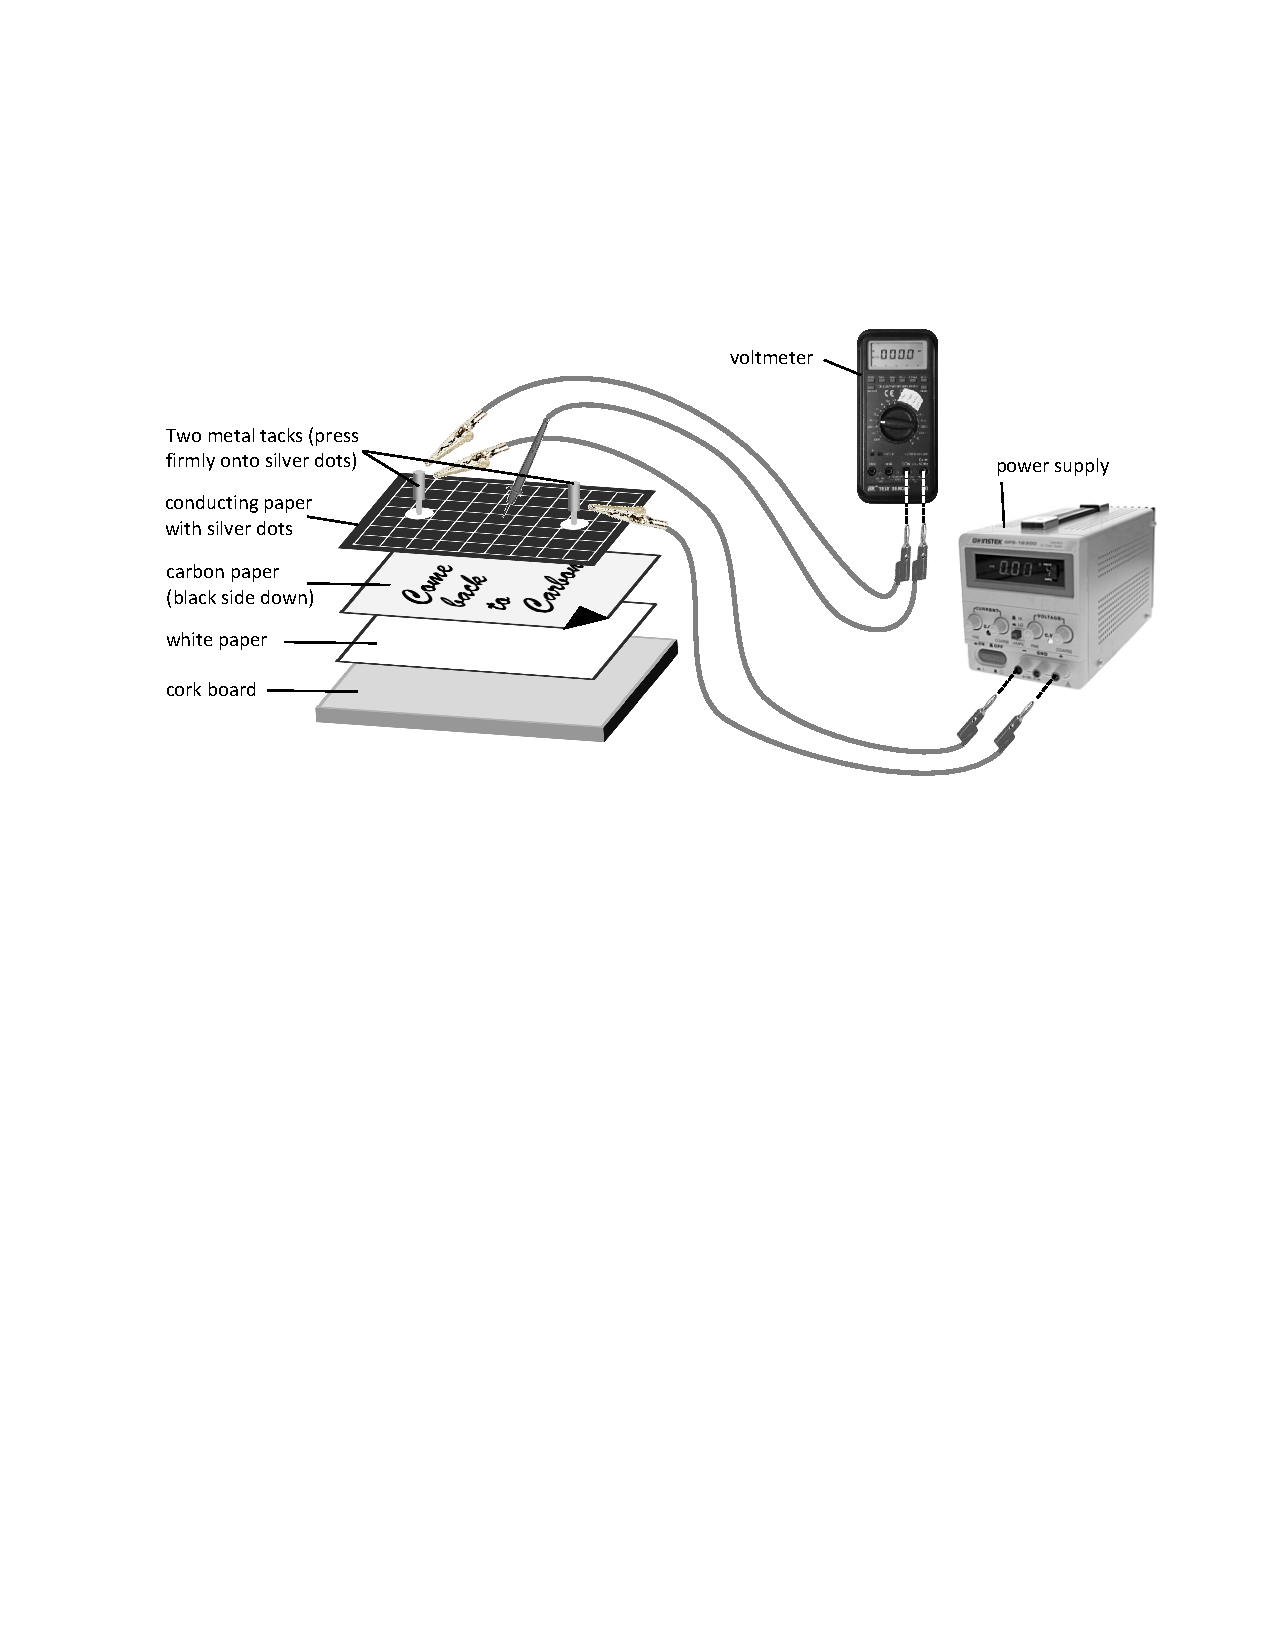
\includegraphics[scale=0.9]{electric_fields_and_equipotential_lines/apparatus_picture.pdf} \par}

%\medskip

\textbf{Introduction}

To help us understand electric forces, we can draw lines of electric field that start at positive charges (pointing directly away from them) and end at negative charges (pointing directly towards them).  


{\setlength{\columnsep}{0.4in}%
\begin{wrapfigure}[11]{r}{2.1in}
\vspace{-0.2in}
{\centering 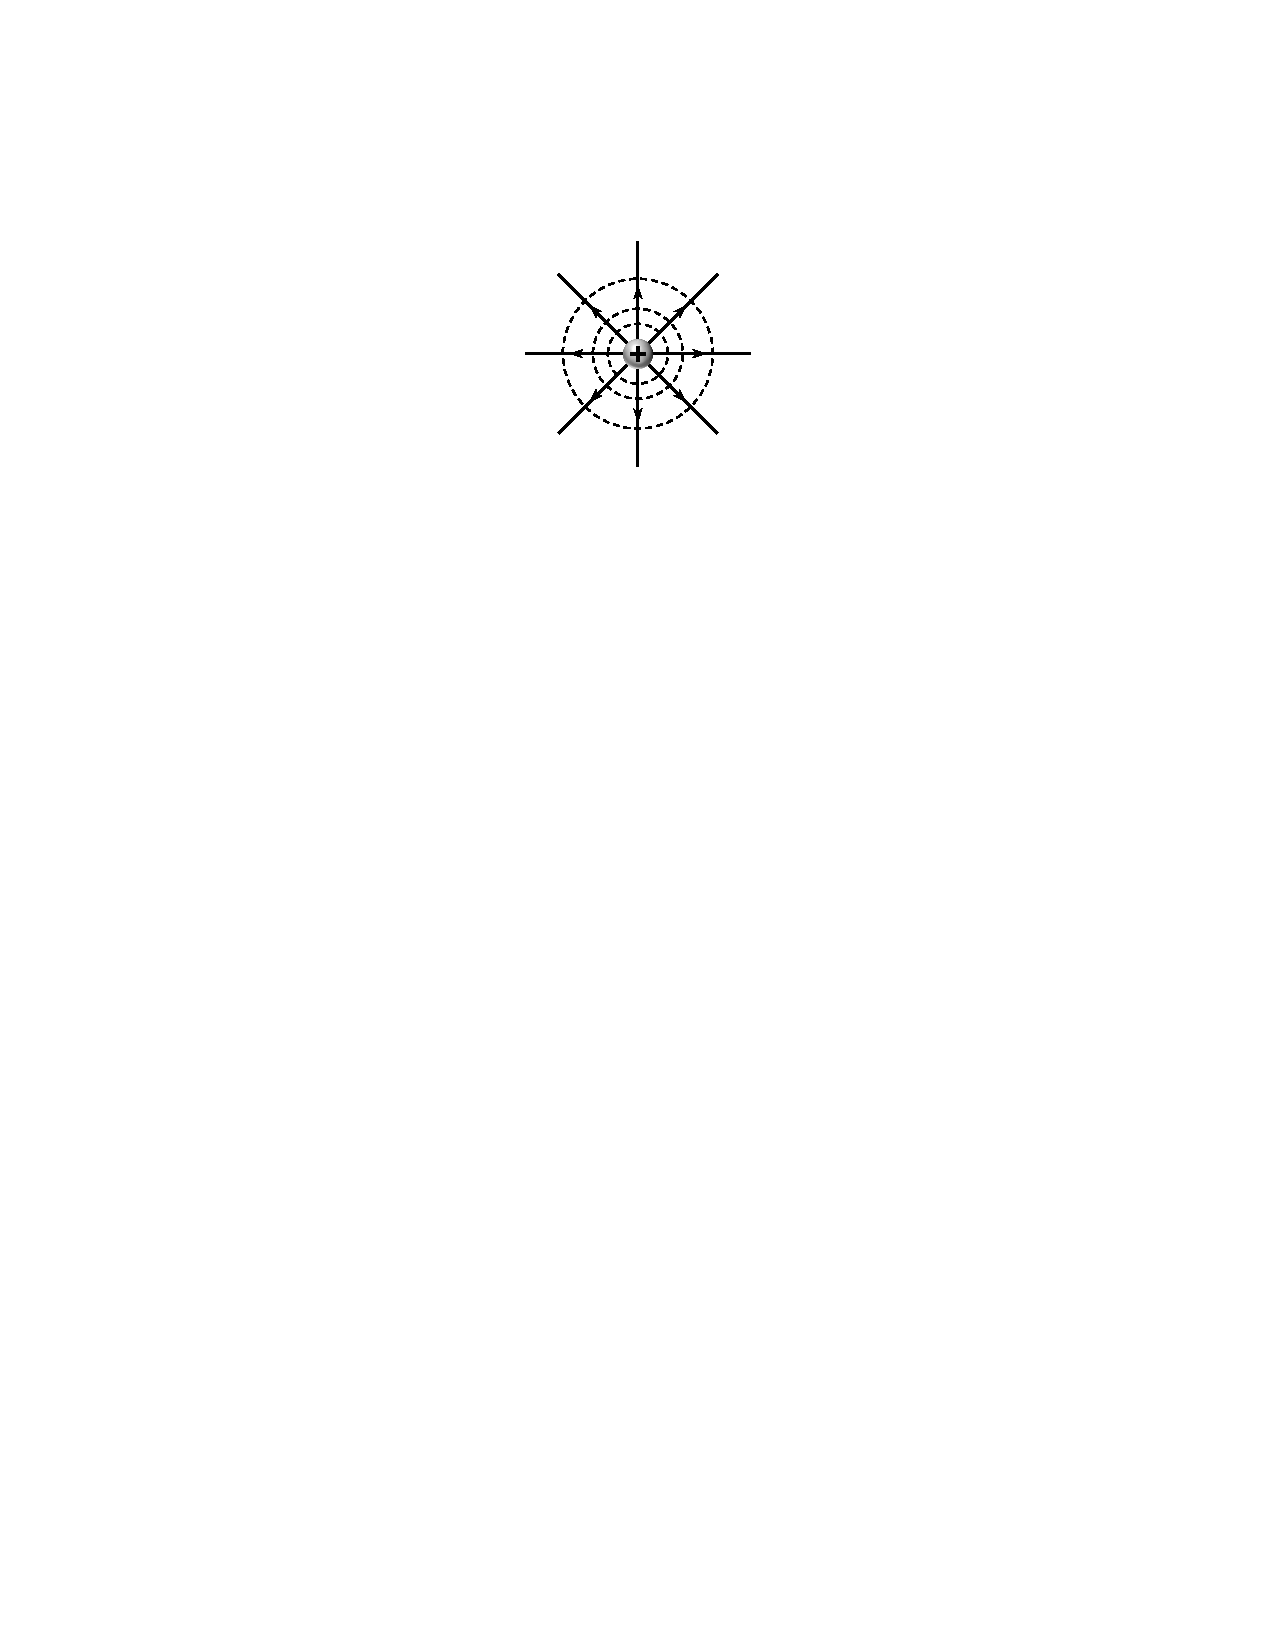
\includegraphics[width=1.7in]{electric_fields_and_equipotential_lines/field_and_potential.pdf} \par}

\textit{\small{A positive charge, with solid arrows showing electric field lines and dashed lines showing equipotentials.}}
\end{wrapfigure}

A charged particle moving along the direction of an electric field line gains or loses potential energy.  We also say that the \textit{electric potential} changes along a field line: the potential decreases going in the same direction as a field line, and the potential increases going in the opposite direction, against a field line.  But there is no change in electric potential in a direction \textit{perpendicular} to electric field lines; paths perpendicular to field lines are called \textit{equipotentials}.

\bigskip

\textbf{Experimental Setup}


Although it is difficult to measure electric field lines directly, you can measure differences in electric potential using a voltmeter.  In this lab, you will use a voltmeter to map out equipotential lines for different configurations of electric field lines.  

}%end of new columnsep

\begin{enumerate}[nosep]
\item Stack a piece of white paper, a piece of carbon paper, and a piece of special conducting paper with two round silver dots onto a cork board, as shown in the diagram above.
\item Push two metal thumbtacks HARD onto the silver dots, so the bottom of each tack is pressed firmly against the silver dot.
\item Use wire leads with alligator clips to connect the two tacks to the positive ($+$) and negative ($-$) terminals of the power supply.  Turn on the power supply and set it to an output of 20 volts.
\item Connect the negative input of the voltmeter (labeled ``COM'') to the same tack as the negative terminal of the power supply.  Connect the positive input of the voltmeter (labeled ``V-$\Omega$'') to the long plastic probe.  For details on how to use your voltmeter, see Appendix \ref{digital_multimeters}.
\end{enumerate}

\pagebreak[2]

\textbf{Activity 1: Field Lines for Two Point Charges}

\begin{enumerate}[labparts]
\item If you haven't already, set up the apparatus as just described.

\item \textit{Prediction:} Draw the electric field lines for two
oppositely charged point particles.  (Remember that field lines start at and point away from positive charges, and they terminate at and point towards negative charges.)  Also sketch the equipotential lines on your drawing, using dotted lines.
\answerspace{2in}

\item \textit{Now do the experiment!}  With your power supply set to 20 volts,
touch the conducting paper with the long probe on your voltmeter, and search around to find 
several points on 
paper registering 16 volts. (For more stable readings, hold the probe at an angle so that more area will be in contact with the conducting paper.)  When you find a place at 16 volts, push down or scratch a little bit 
so that the middle sheet of carbon paper will make marks on the bottom sheet of white paper---you 
can peak underneath to check.
\textit{You should be able to do this without puncturing the conducting paper.  Please don't poke holes, so the conducting paper can be reused!}

\item Repeat for 12 volts, 8 volts, and 4 volts.

\item You should end up with a series of dots on your sheet of paper. Connect
those associated with the same potential with smooth lines. Label each line 
with its associated voltage.  Attach a copy of the sheet with your measurements to this lab.
Draw a sketch of your results below.
\answerspace{2in}

\item Recalling the relationship between electric field lines and equipotential
lines, sketch in the electric field lines on the drawing you just made. 

\item Does your experimental result agree with your prediction? Explain.
\answerspace{1in}

\end{enumerate}

\pagebreak[2]
\textbf{Activity 2: Field Lines for Two Parallel Plates}

For static electric charges (when charges are not moving), the 
electric field within a conductor is zero, and electric field lines leave \textit{perpendicular} to a conductor's surface.  
In this activity, you will examine the field lines and equipotentials for two parallel conducting lines.  This situation is the two-dimensional analog of a pair of parallel conducting plates, also called a ``parallel plate capacitor.''

\begin{enumerate}[labparts]
\item \textit{Prediction:} Draw what you predict the field lines and equipotential
lines between two parallel plates will look like.
\answerspace{1.8in}

\item Set up your apparatus again, this time using the conducting paper with two silver parallel lines drawn on it.  Again, be sure to press the thumbtacks firmly down onto the silver conducting lines.  Carry out the instructions from Activity 1 to check your prediction above.  Attach a copy of the sheet with your measurements to this lab.
Draw a sketch of your results below, including equipotentials and field lines.
\answerspace{1.8in}

\item Does your result agree with your prediction? Explain.
\answerspace{.5in}

\end{enumerate}
\textbf{Activity 3: Field Lines Between a Point Charge and a Plate}

\begin{enumerate}[labparts]

\item Draw what you \textit{predict} the field lines and equipotential
lines between a point charge and a parallel plate will look like.
\answerspace{1.8in}

\item Map the field lines as before, attach a copy of the sheet with your measurements to this lab, and draw a sketch of your results below.
\answerspace{1.8in}

\item Does your result agree with your prediction? Explain.
\answerspace{.8in}

%\item If the potential is zero, must the electric field be zero as well?
%\answerspace{.3in}
%\item What can you say about the electric field along an equipotential line?\vspace{15mm}

\end{enumerate}
%\textbf{Activity 4: Field Lines for a Plate and a Charged Circle}

%\textbf{Prediction:} Sketch what you think the field and potential
%lines between a charged circle and a plate look like.
%\vspace{1in}

%\begin{enumerate}
%\item Determine the field lines.
%\item What is the field strength within a charged, continuous surface?\vspace{15mm}
%\end{enumerate}

